\title{Report of Large Amplitude Pendulum Experiment} % Title, modify to the name of experiment
\author{Haopeng Chen}% Author, modify to your name
\date{October 26th, 2021}% Date, Modify to the DATE of EXPERIMENT


\documentclass[12pt]{article}
\usepackage{graphicx}
\usepackage{makecell}
\usepackage{float}
\newcommand{\diff}{\,\mathrm{d}}
\usepackage[margin=1in]{geometry}
\usepackage{fancyhdr}
\pagestyle{fancy}
\usepackage{extarrows}
\usepackage{breqn}
\usepackage[colorlinks,linkcolor=blue]{hyperref}
\newcommand{\N}{\mathbb{N}}
\newcommand{\Z}{\mathbb{Z}}
\newcommand{\trans}{^{\mathrm T}}
\usepackage[table]{xcolor}
\usepackage{bm}
\usepackage{array}
\usepackage[english]{babel}
\usepackage{natbib}
\usepackage{url}
\graphicspath{{images/}}
\usepackage{parskip}
\usepackage{fancyhdr}
\usepackage{vmargin}
\usepackage[font={bf, footnotesize}, textfont=md]{caption}
\usepackage{amsmath,amsthm,amssymb}
\usepackage{indentfirst}
\usepackage{bookmark}
\usepackage{fontspec}
\setmainfont{TeX Gyre Termes}
\setsansfont{TeX Gyre Heros}
\setmonofont{JetBrains Mono NL}
\usepackage{mathtools}
\usepackage{unicode-math}
\setmathrm{XITS Math}
\setmathsf{XITS Math}
\usepackage{listings}
\usepackage{ctex}

% 用来设置附录中代码的样式

\lstset{
    basicstyle          =   \ttfamily,
    keywordstyle        =   \ttfamily,
    commentstyle        =   \rmfamily\itshape,
    stringstyle         =   \ttfamily,
    % flexiblecolumns,
    numbers             =   left,
    showspaces          =   false,
    numberstyle         =   \ttfamily,
    showstringspaces    =   false,
    captionpos          =   t,
    frame               =   lrtb,
}

\lstdefinestyle{Python}{
    language        =   Python,
    basicstyle      =   \ttfamily,
    numberstyle     =   \ttfamily,
    keywordstyle    =   \color{blue},
    commentstyle    =   \color{green}\ttfamily,
    breaklines      =   true,
    % columns         =   fixed,
    basewidth       =   0.5em,
}





\newenvironment{theorem}[2][Theorem]{\begin{trivlist}
                \item[\hskip \labelsep {\bfseries #1}\hskip \labelsep {\bfseries #2.}]}{\end{trivlist}}
\newenvironment{lemma}[2][Lemma]{\begin{trivlist}
                \item[\hskip \labelsep {\bfseries #1}\hskip \labelsep {\bfseries #2.}]}{\end{trivlist}}
\newenvironment{exercise}[2][Exercise]{\begin{trivlist}
                \item[\hskip \labelsep {\bfseries #1}\hskip \labelsep {\bfseries #2.}]}{\end{trivlist}}
\newenvironment{reflection}[2][Reflection]{\begin{trivlist}
                \item[\hskip \labelsep {\bfseries #1}\hskip \labelsep {\bfseries #2.}]}{\end{trivlist}}
\newenvironment{proposition}[2][Proposition]{\begin{trivlist}
                \item[\hskip \labelsep {\bfseries #1}\hskip \labelsep {\bfseries #2.}]}{\end{trivlist}}
\newenvironment{corollary}[2][Corollary]{\begin{trivlist}
                \item[\hskip \labelsep {\bfseries #1}\hskip \labelsep {\bfseries #2.}]}{\end{trivlist}}
\DeclareMathOperator{\tr}{tr}
\DeclareMathOperator{\rank}{rank}
\DeclareMathOperator{\Span}{span}
\DeclareMathOperator{\row}{row}
\DeclareMathOperator{\col}{col}
\DeclareMathOperator{\range}{range}
\DeclarePairedDelimiterX{\inp}[2]{\langle}{\rangle}{#1, #2}
\DeclareMathOperator{\Proj}{Proj}
\DeclareMathOperator{\trace}{trace}
\newcommand{\Her}{^{\mathrm H}}
\DeclareMathOperator{\diag}{diag}
\makeatletter
\newcommand\fcaption{\def\@captype{table}\caption}
\makeatother
\setmarginsrb{3 cm}{2.5 cm}{3 cm}{2.5 cm}{1 cm}{1.5 cm}{1 cm}{1.5 cm}


\makeatletter
\let\thetitle\@title
\let\theauthor\@author
\let\thedate\@date
\makeatother

\pagestyle{fancy}
\fancyhf{}
\rhead{\theauthor}
\lhead{\thetitle}
\cfoot{\thepage}

\begin{document}


\begin{titlepage}
  \centering
  \vspace*{0.5 cm}
  
\includegraphics[scale = 0.75,width=6cm]{CUHK}\\[1.0 cm]   % University Logo
  \textnormal{\large The Chinese University of Hong Kong, Shenzhen}\\[2.0 cm]
  \textnormal{\Large PHY 1002}\\[0.5 cm]
  \textnormal{\large Physics Laboratory}\\[0.5 cm]               % Course Name
  \rule{\linewidth}{0.2 mm} \\[0.4 cm]
  { \huge \bfseries \thetitle}\\
  \rule{\linewidth}{0.2 mm} \\[1.5 cm]

  \begin{minipage}{0.4\textwidth}
    \begin{flushleft} \large
      \emph{Author:}\\
      \theauthor
    \end{flushleft}
  \end{minipage}
  \begin{minipage}{0.4\textwidth}
    \begin{flushright} \large
      \emph{Student Number:} \\
      120090645  % Modify to your student number
    \end{flushright}
  \end{minipage}\\[2 cm]
  {\large \thedate}\\[2 cm]

  \vfill

\end{titlepage}

\tableofcontents
\pagebreak

\parindent=0.5in
\rmfamily

% Introduction
\section{Introduction:}
A pendulum is a weight suspended from a pivot so that it can swing freely. When a pendulum is displaced sideways from its resting, equilibrium position, it is subject to a restoring force due to gravity that will accelerate it back toward the equilibrium position. When released, the restoring force acting on the pendulum's mass causes it to oscillate about the equilibrium position, swinging back and forth. The time for one complete cycle, a left swing and a right swing, is called the period. The period depends on the length of the pendulum and also to a slight degree on the amplitude, the width of the pendulum's swing. Simple Pendulum is one of the most common phenomenon in our daily life. During the development of Physics, it has drawn a large amount of attention from physicists and been studied for a long time. \par
This is an experiment to figure out the difference between \emph{Large Amplitude Pendulum} and \emph{Small Amplitude Pendulum}. Therefore, a series of three experiments are conducted to explore the dependence of the period of a simple pendulum on the amplitude of the oscillation. Also, we manage to plot the graph of the angular displacement, angular velocity, and angular acceleration versus time for large amplitude to show the difference from the sinusoidal motion of low amplitude oscillations. We are going to use fundamental calculus to quantitatively figure out the relation between the angular displacement, angular velocity, and angular acceleration curves.

% Theory overview
\section{Theory:}
For a small amplitude physical pendulum, its period is approximately given by
\begin{equation}\label{eq:1}
  T_0=2\pi\sqrt{\frac{I}{mgd}}
\end{equation}
where $I$ is the rotational inertia of the pendulum about the pivot point, $m$ is the total mass of the pendulum, and $d$ is the distance from the pivot to the the center of the mass. The approximation becomes more exact as the amplitude goes to zero. With this limit, the motion is simple harmonic and the angular displacement is given by
\begin{equation}\label{eq:2}
  \theta=\theta_0\sin(At+\phi)
\end{equation}
where $\theta_0$ is the initial angular displacement, $A=\frac{2\pi}{T_0}$ is a constant, representing the angular frequency, and $\phi$ is the phase angle which is determined by the value of $\theta$ when $t=0$. It is thereby a constant. Then, by calculus, we can point out the angular velocity and angular acceleration
\begin{equation}\label{eq:3}
  \omega=\frac{d\theta}{dt}=A\theta_0\cos(At+\phi)
\end{equation}
\begin{equation}\label{eq:4}
  \alpha=\frac{d\omega}{dt}=-A^2\theta_0\sin(At+\phi)
\end{equation}
\par
However, things change a lot in large amplitude. If we continue to use the approximation equations above, we will miss in errors. So, we need a more accurate one. For larger amplitudes, the restoring torque is not linear and the period is given by an infinite series
\begin{equation}\label{eq:5}
  T=T_0[1+\sum_{n = 1}^{\infty}(\frac{(2n-1)!!}{2^nn!})^2\sin^{2n}(\frac{A}{2})]
\end{equation}
where $A$ (same as the $\theta_0$ in Equation \refeq{eq:2}, Equation \refeq{eq:3} and Equation \refeq{eq:4}) is the oscillation amplitude. Consider its first five terms and we have
\begin{equation}\label{eq:6}
  T\approx{T_0[1+(\frac{1}{2})^2\sin^2({\frac{A}{2}})+({\frac{3}{8}})^2\sin^4({\frac{A}{2}})+({\frac{15}{48}})^2\sin^6({\frac{A}{2}})+({\frac{105}{384}})^2\sin^8({\frac{A}{2}})]}
\end{equation}

% Illustrate the Experiment Procedure
\section{Experiment Process:}
The following illustrates the facility of experiment and details of the experiment approaches.

% Setup part
\subsection{Equipment Setup}
First, we thread the metal rod into the iron base and attach the rotary motion sensor on it. Attach the rotary motion sensor to one \textit{Paspot} input on the PASCO 850 Universal Interface. Then, we remove the silver thumbscrew to install the pulley to the rotary motion sensor. We make the large step of the pulley towards out on the rotary motion sensor and attach the pendulum rod at its \emph{center} using another longer thumbscrew which matches the rod perfectly. The rod is positioned so the bumps on the pulley hold it in place. At last, we attach two brass masses on the each end of the rod. One is even with the end, while the other is left about $3$cm to it. As shown in Figure \ref{figSetup}.
\begin{figure}[H]
  \centering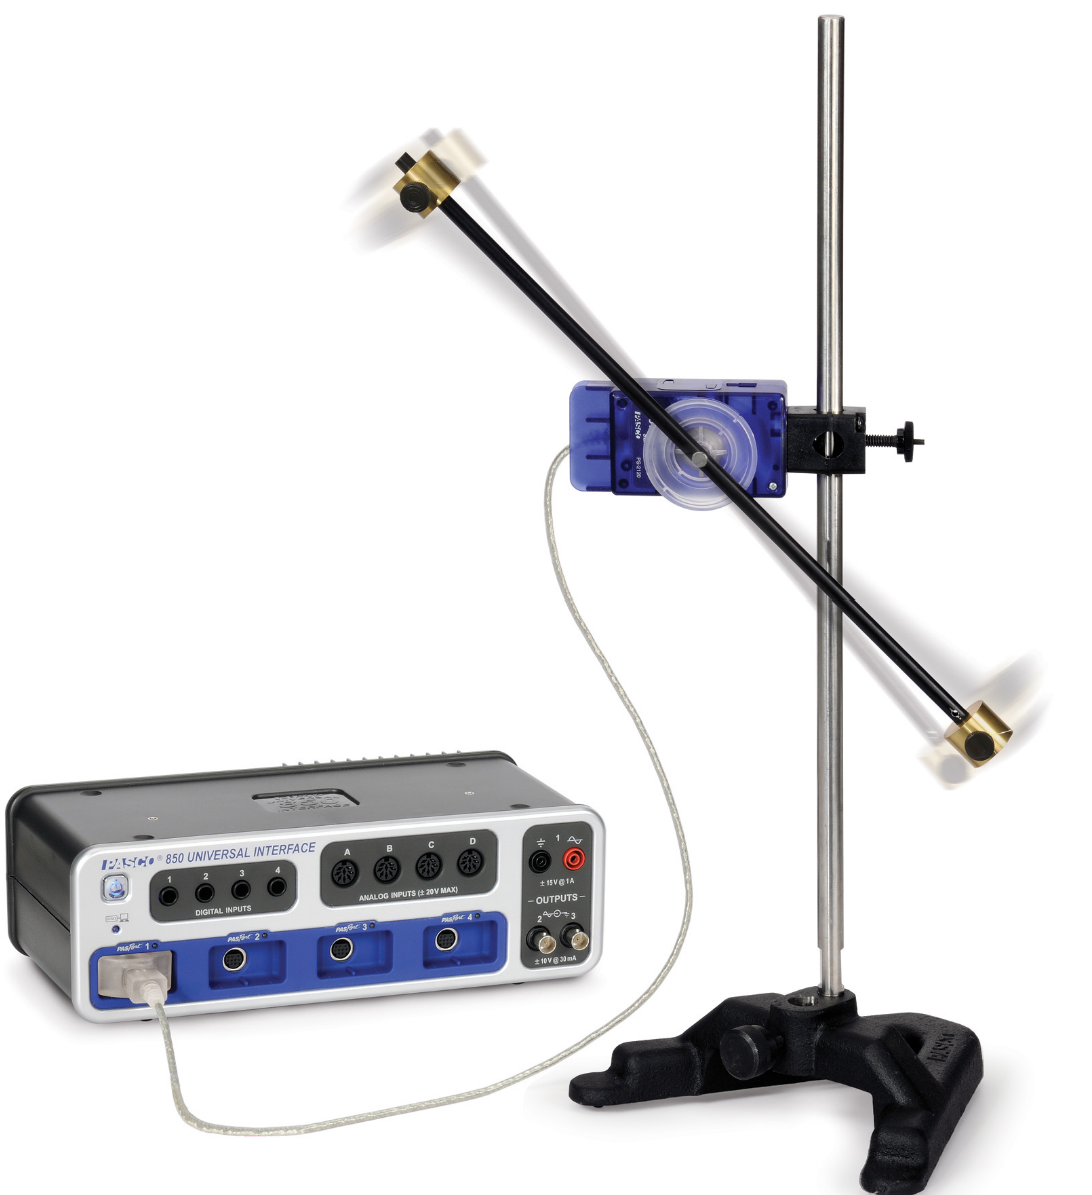
\includegraphics[width=5.2cm]{figSetup.png}
  \caption{Experiment 1 Setup}
  \label{figSetup}
\end{figure}

% experiment 1 procedure
\subsection{Qualitative Analysis}
In this experiment, the rotary motion sensor is at $100$Hz.\par
For \emph{small pendulum}, we first make sure the pendulum rests at its equilibrium position. We click the \textit{RECORD} button in PASCO Capstone\texttrademark to initialize the rotary motion sensor, making its start point to origin. Then, we displace the pendulum at an angle less than $20^\circ$ (about $0.35$rad) from equilibrium. Release the pendulum and click \textit{STOP} after a few oscillations. Then, we have the data shown in \emph{Figure 2}, \emph{Figure 3} and \emph{Figure 4}.\par
For \emph{large pendulum}, we repeat the previous steps but displace the pendulum nearly $180^\circ$ from equilibrium.

% Experiment 2 procedure
\subsection{Quantitative Analysis of Small Amplitude Oscillations}
In this experiment, the rotary motion sensor is at $100$Hz.\par
Before we start, we first slide down the upper mass until it is touching the pulley. And we use the thumbscrew to hold it at that place. Likely, we first click \textit{RECORD} with the pendulum resting at its equilibrium position, initializing the sensor to start at the origin. Then, we displace the pendulum less than $5^\circ$ (about $0.10$rad) from equilibrium. Release it and click \textit{STOP} after $13$ oscillations.

% Experiment 3 Procedure
\subsection{Quantitative Analysis of Large Amplitude Oscillations}
In this experiment, the theory motion sensor is at $200$Hz.\par
Similarly, we first click \textit{RECORD} with the pendulum resting at its equilibrium position, initializing the sensor to start at the origin. Then, we displace the pendulum at about $10^\circ$ (about $0.20$rad) from equilibrium. Release it and click \textit{STOP} after $3$ oscillations.

% Experiment Raw Data
\section{Raw Data:}
% Figures
\subsection{Raw Data Figures}
\begin{figure}[H]
  \centering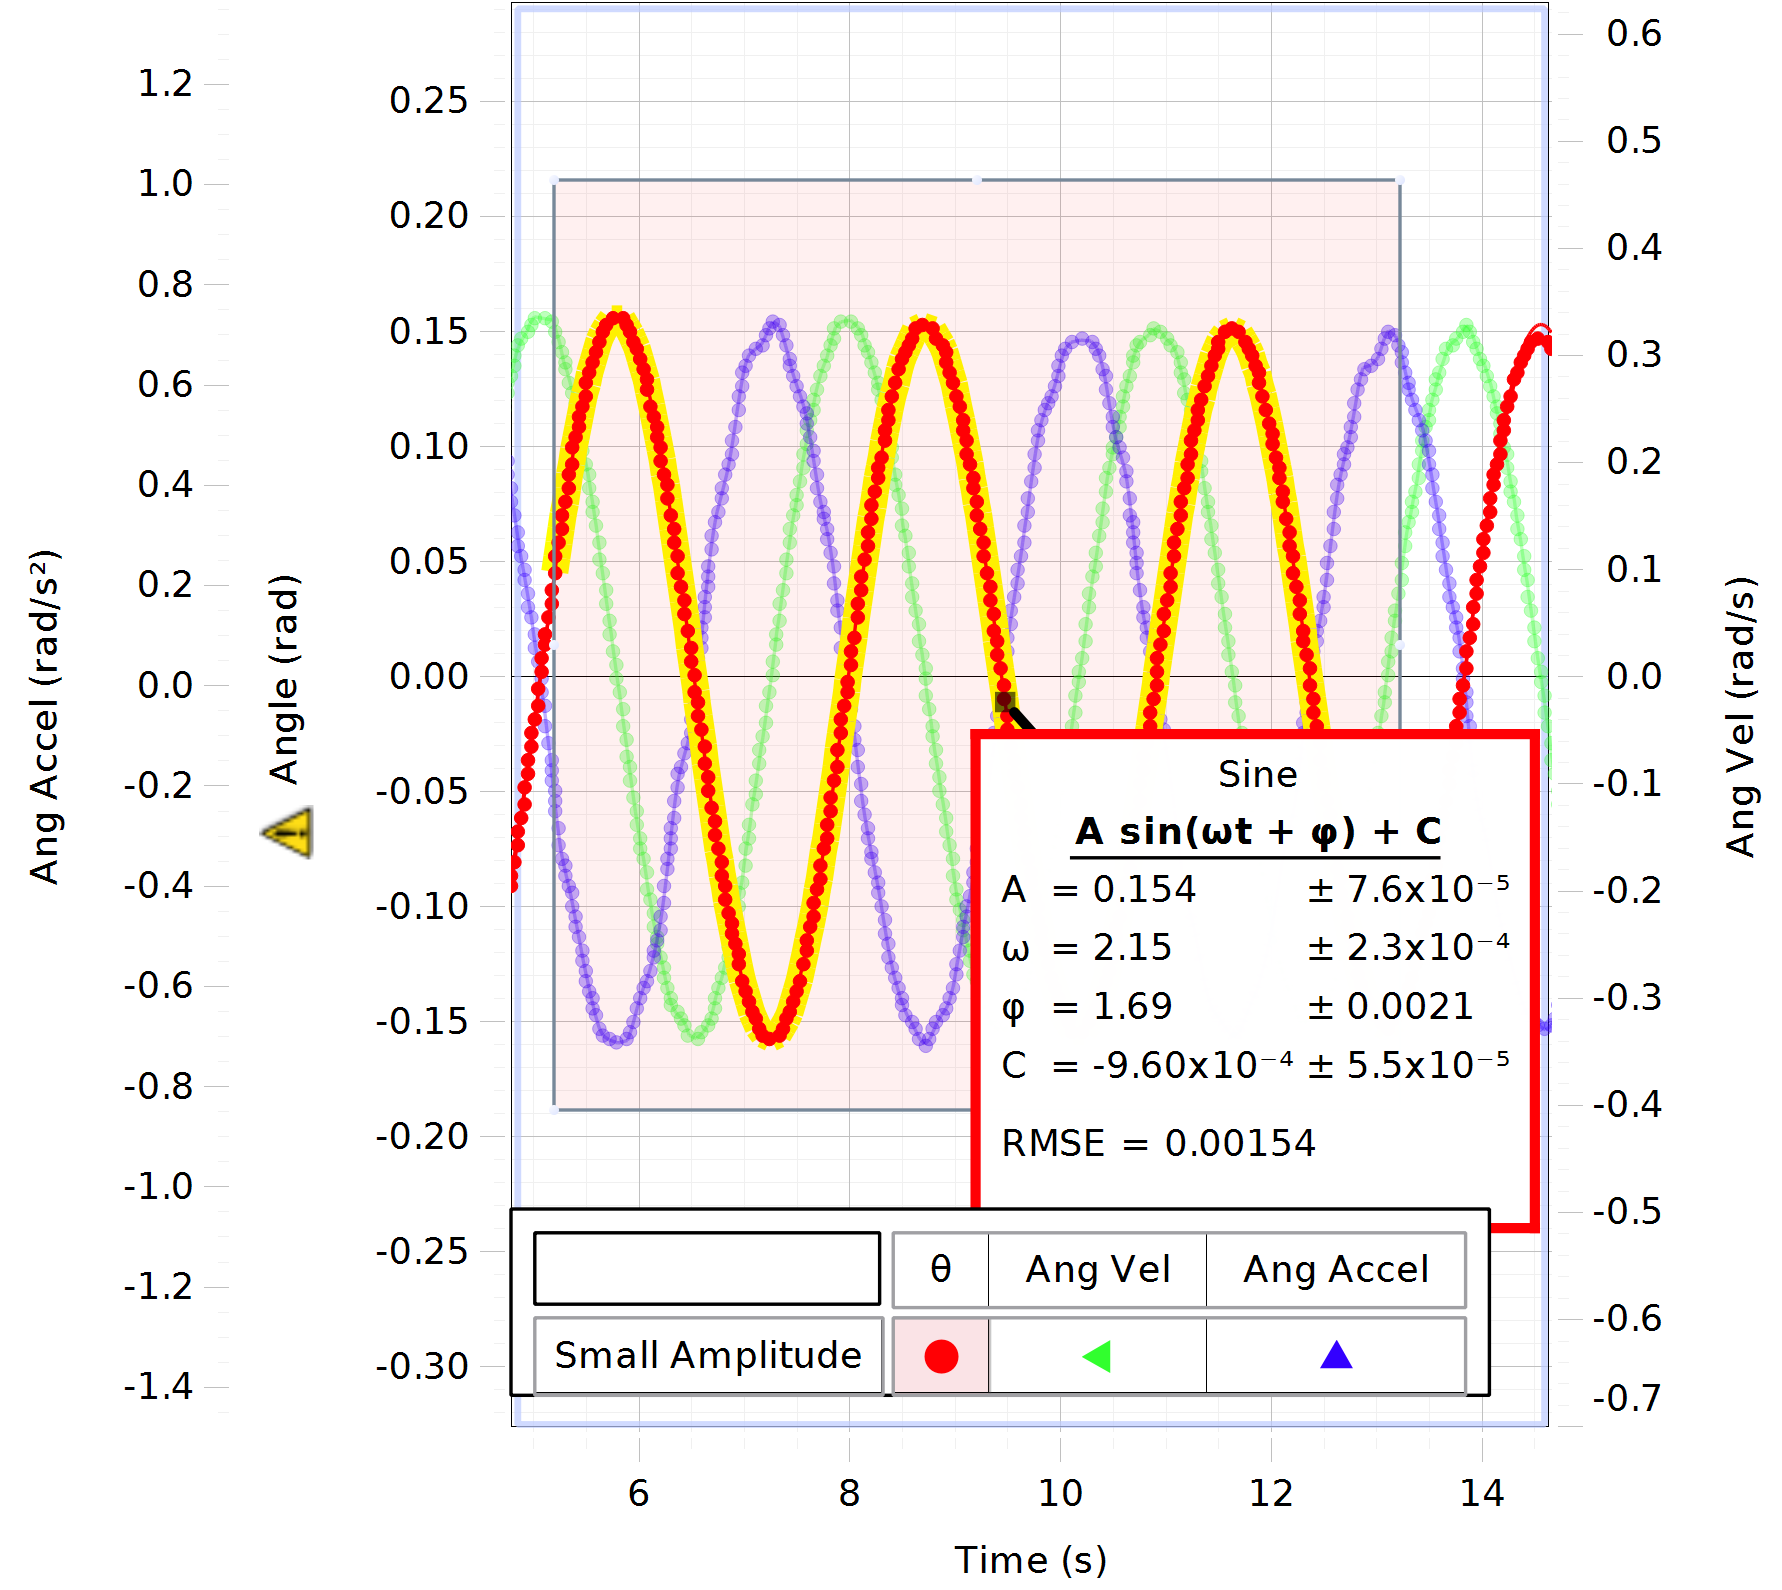
\includegraphics[width=15cm]{figQualitativeSmallAngle.png}
  \caption{Sine Curve Approximation of Angular Magnitude in Qualitative Analysis for Small Amplitude}
  \label{figAngleQualitativeSmallAngle}
\end{figure}
\begin{figure}[H]
  \centering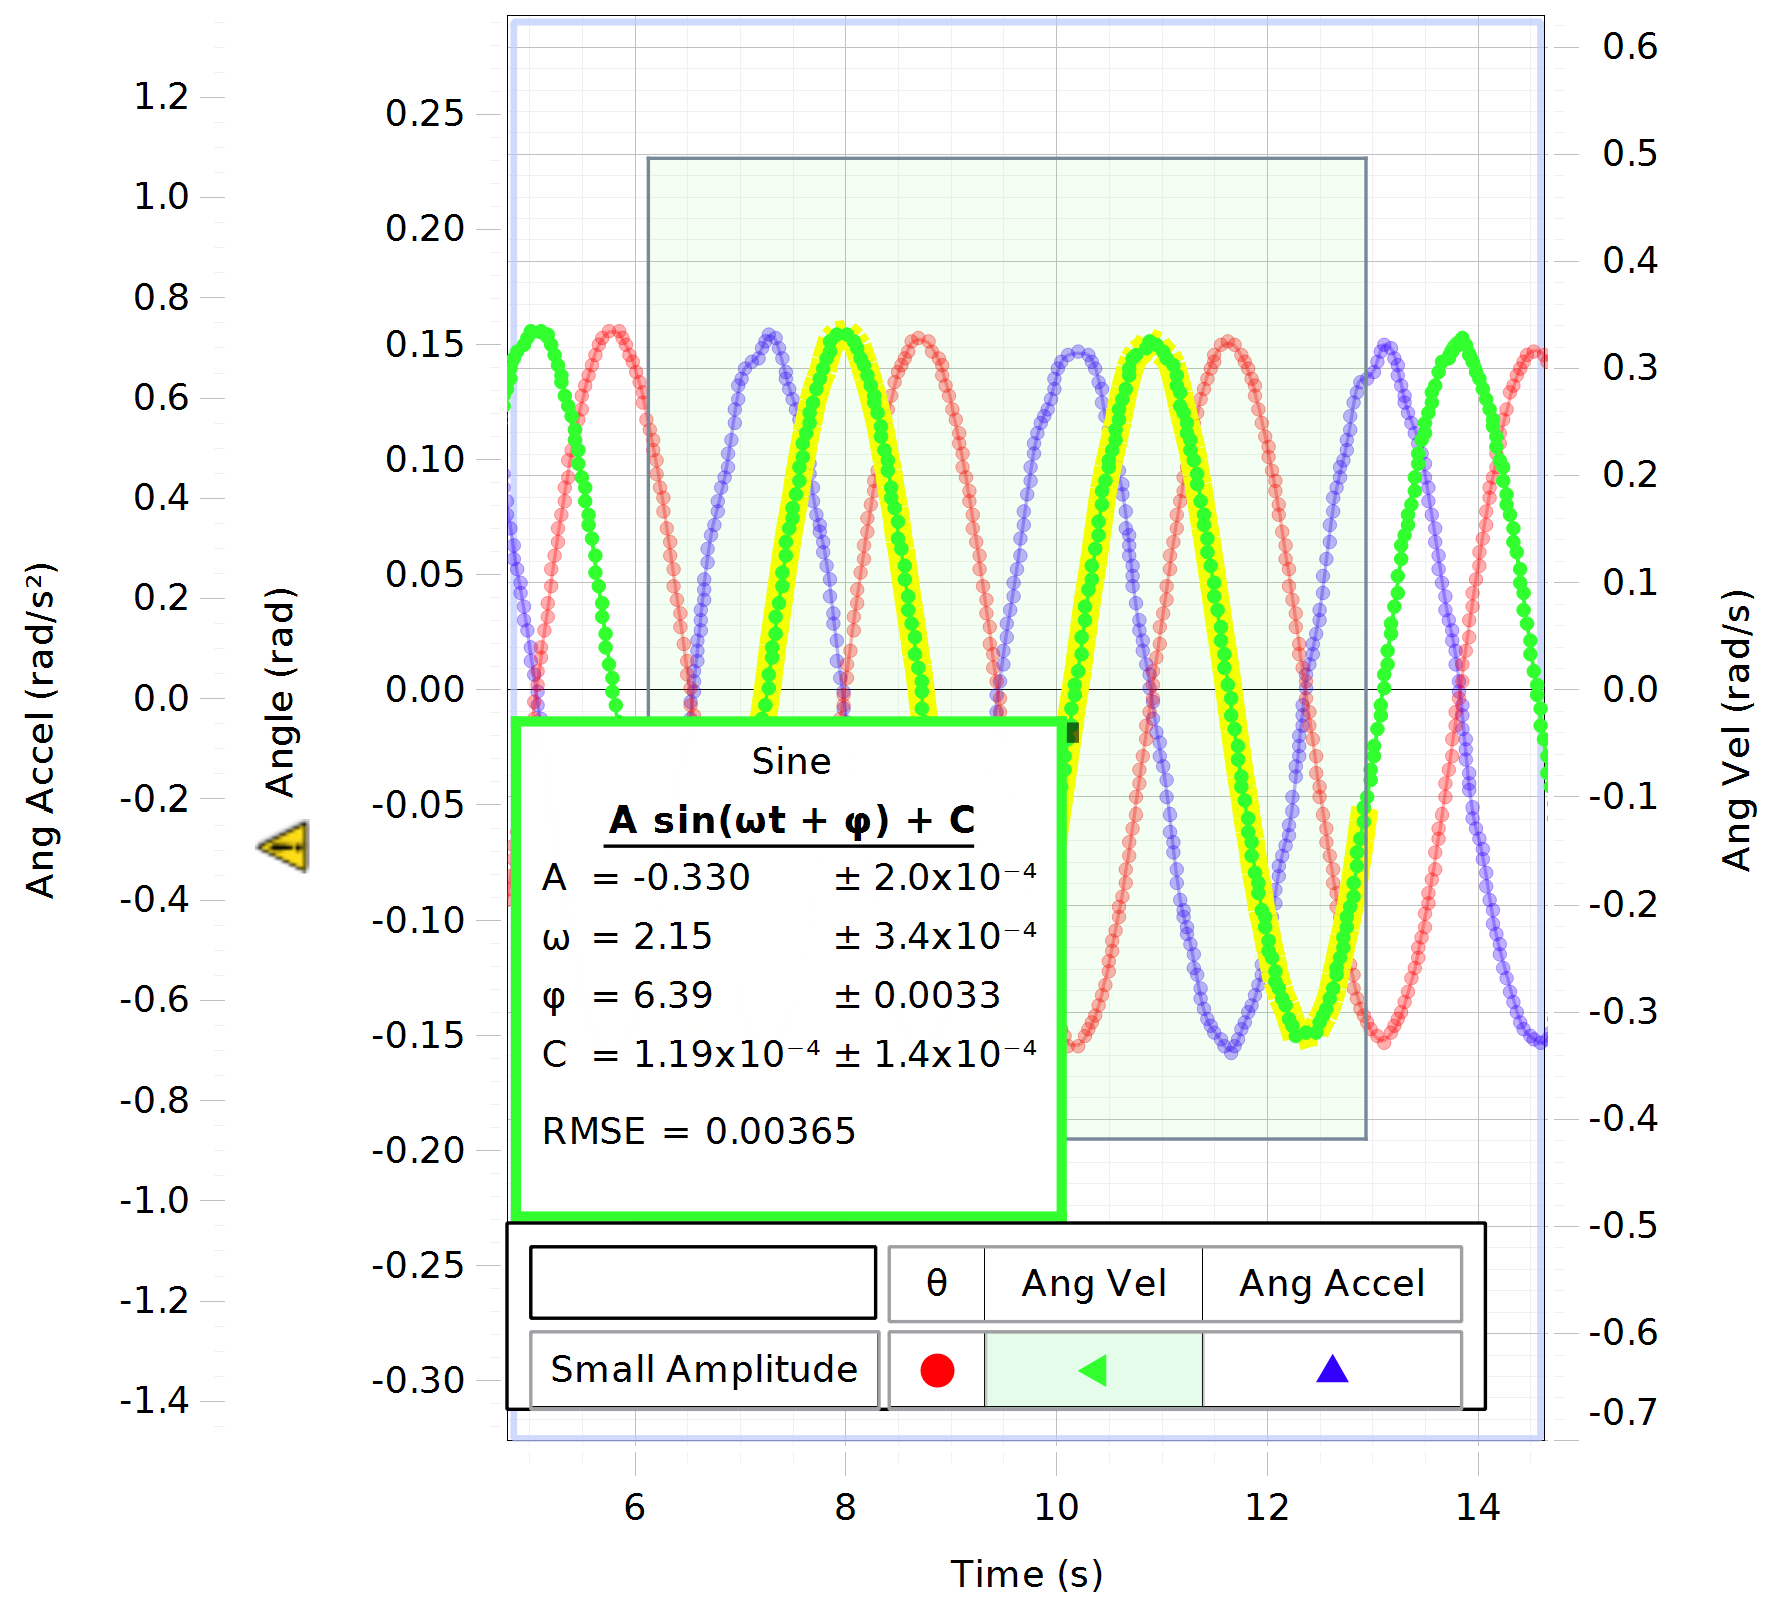
\includegraphics[width=15cm]{figQualitativeSmallAngle2.png}
  \caption{Sine Curve Approximation of Angular Velocity in Qualitative Analysis for Small Amplitude}
  \label{figAngleVelQualitativeSmallAngle}
\end{figure}
\begin{figure}[H]
  \centering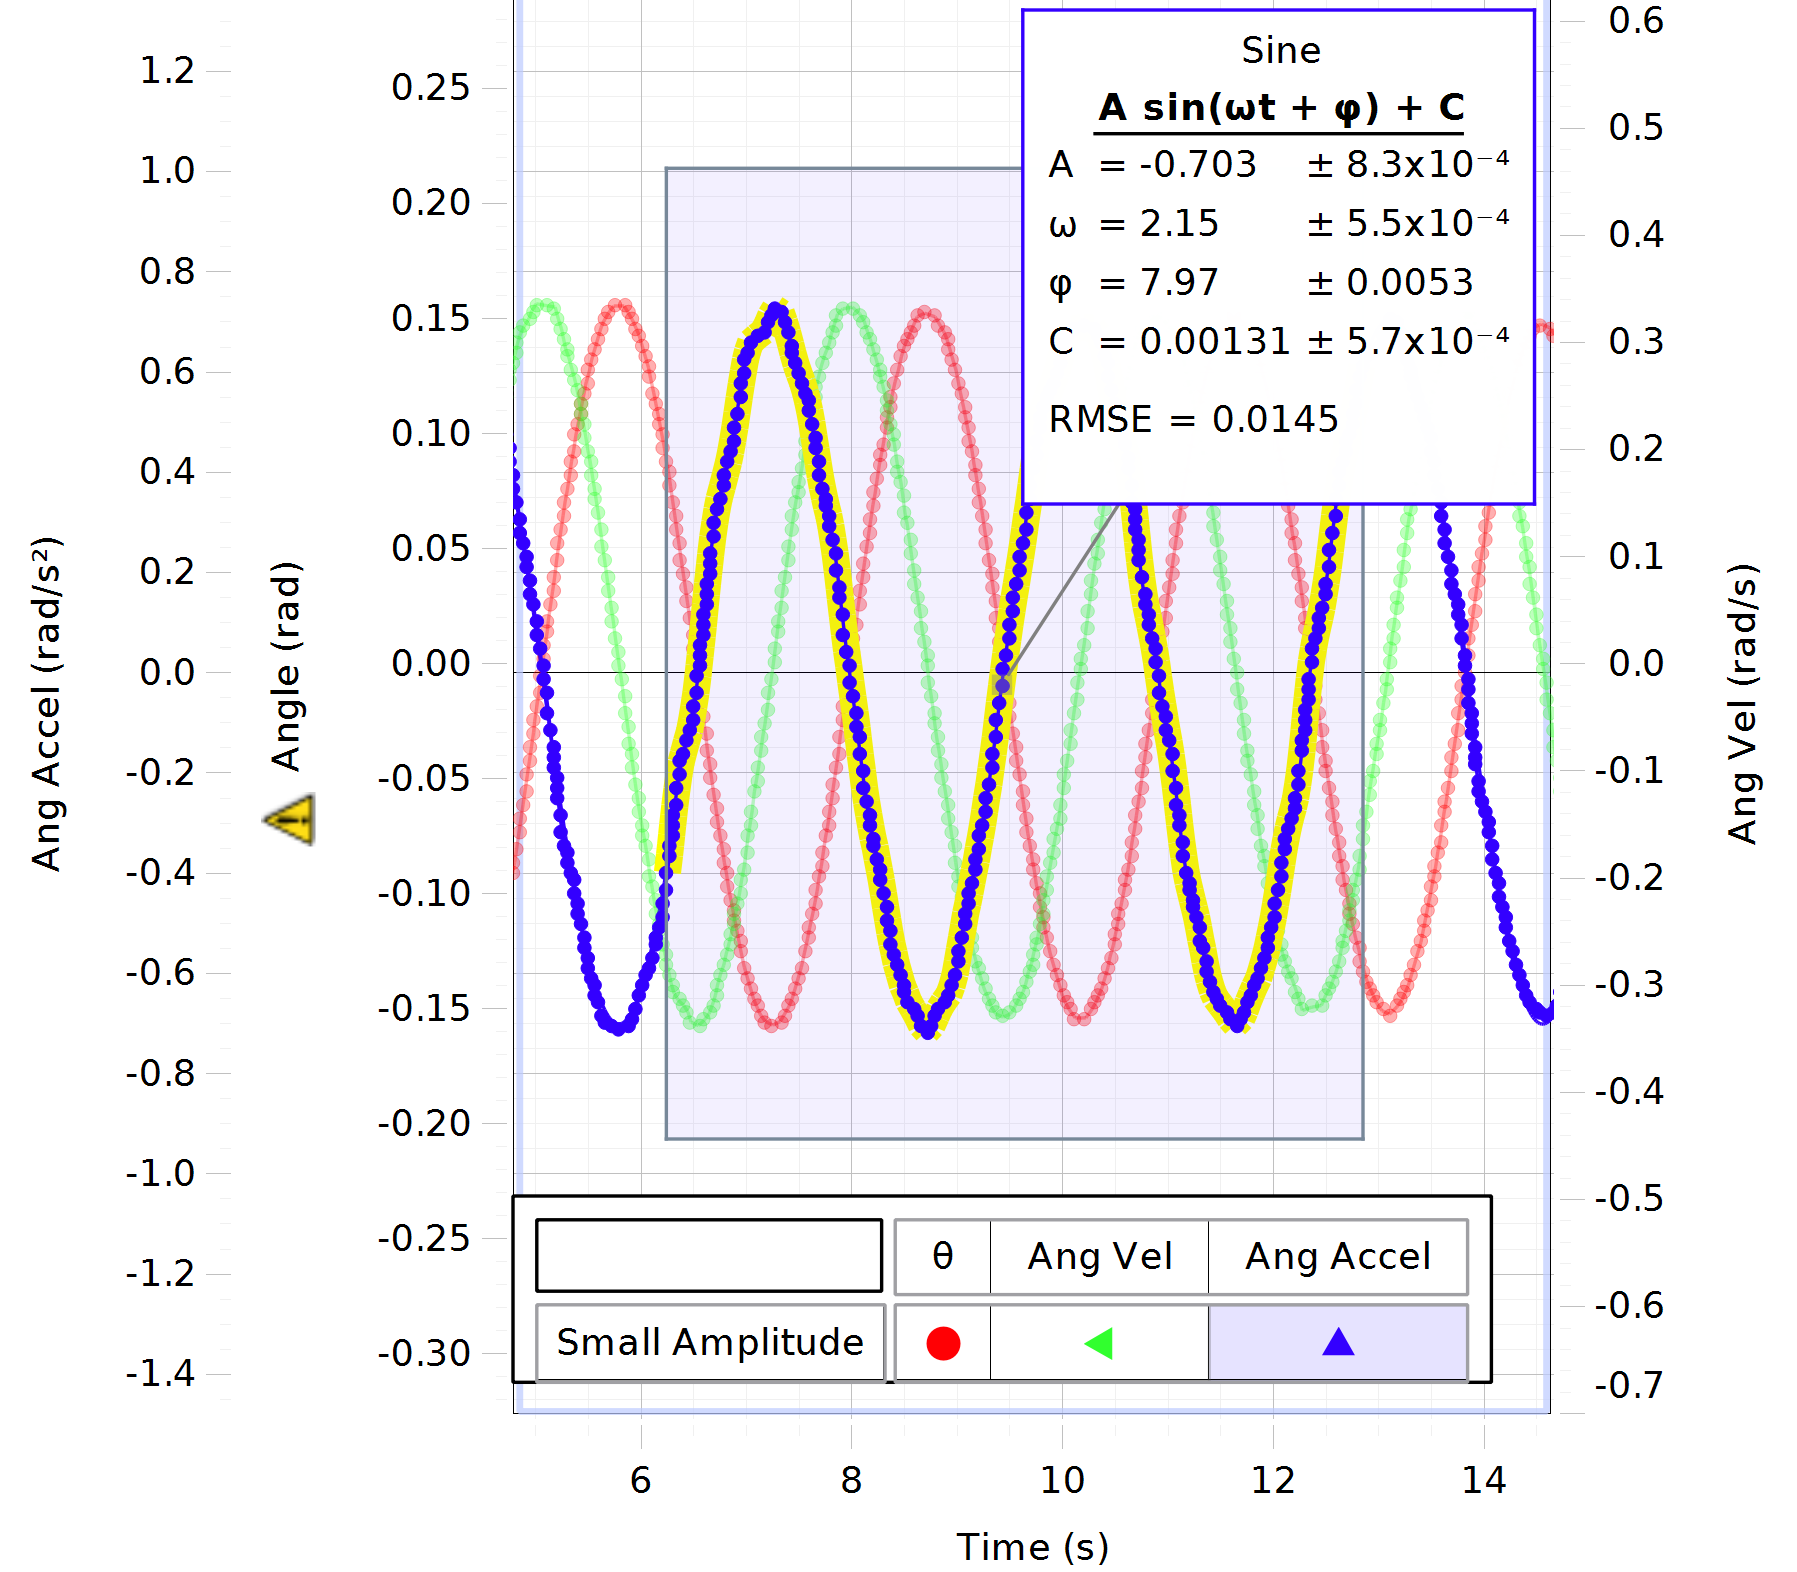
\includegraphics[width=15cm]{figQualitativeSmallAngle3.png}
  \caption{Sine Curve Approximation of Angular Acceleration in Qualitative Analysis for Small Amplitude}
  \label{figAngleAccelQualitativeSmallAngle}
\end{figure}
\begin{figure}[H]
  \centering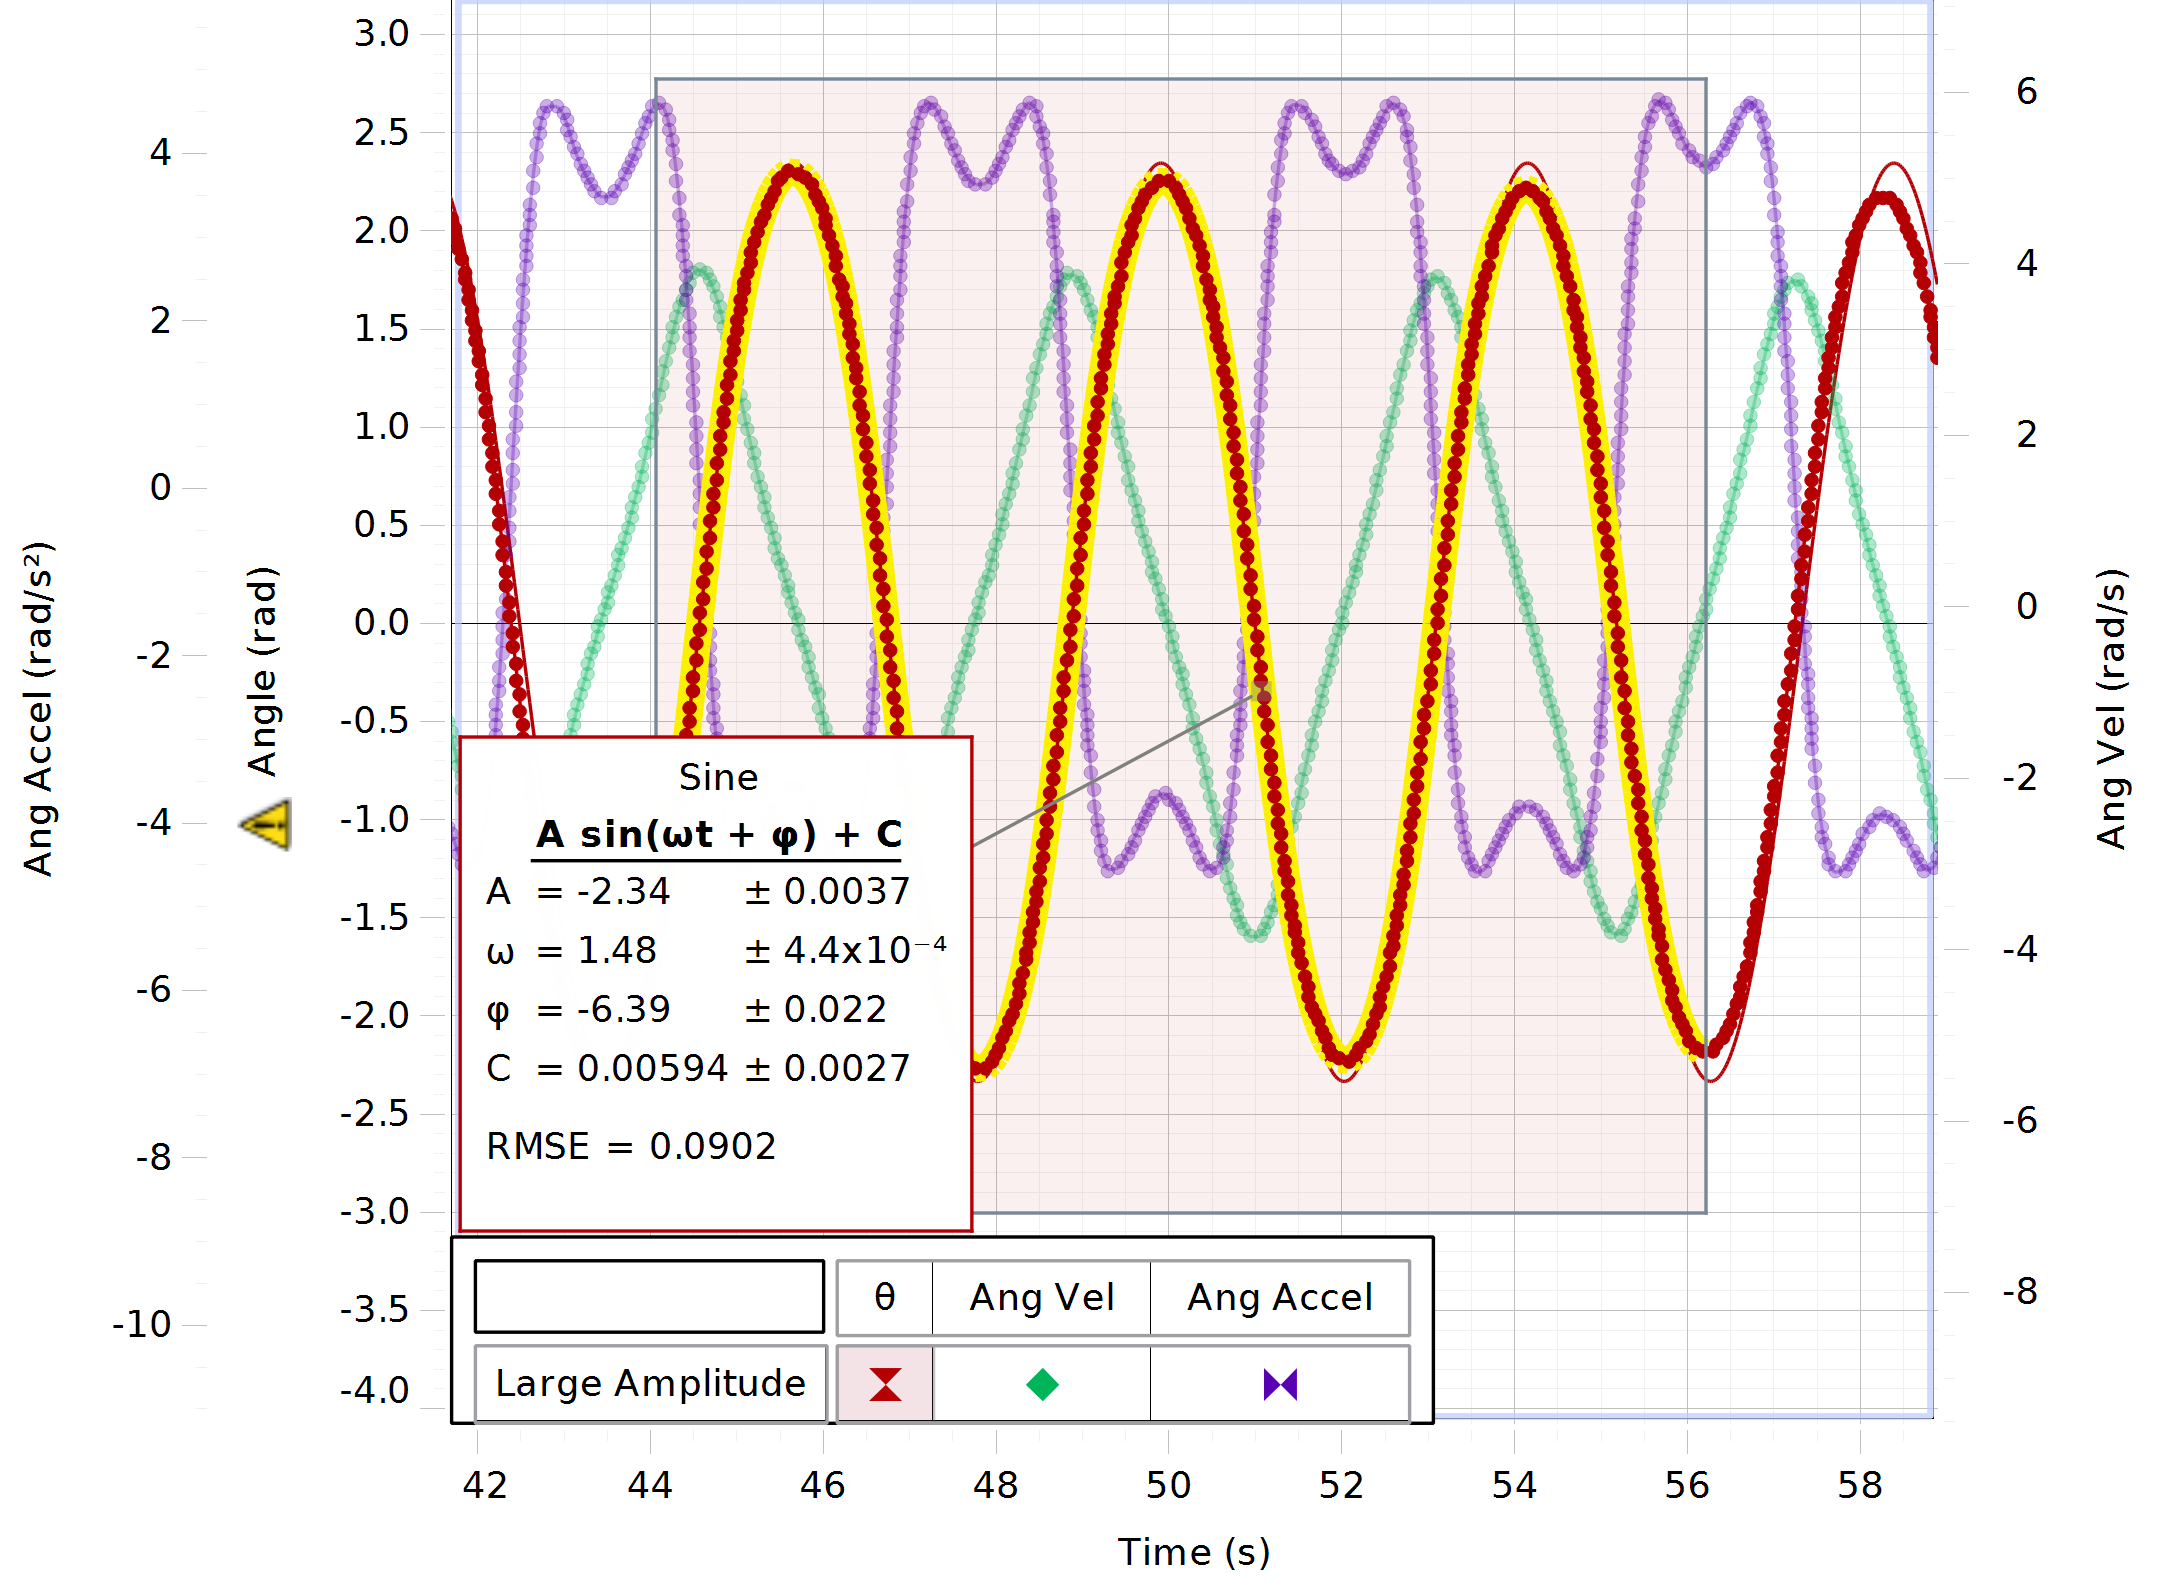
\includegraphics[width=15cm]{figQualitativeLargeAngle.png}
  \caption{Sine Curve Approximation of Angular Magnitude in Qualitative Analysis for Large Amplitude}
  \label{figAngleQualitativeLargeAngle}
\end{figure}
\begin{figure}[H]
  \centering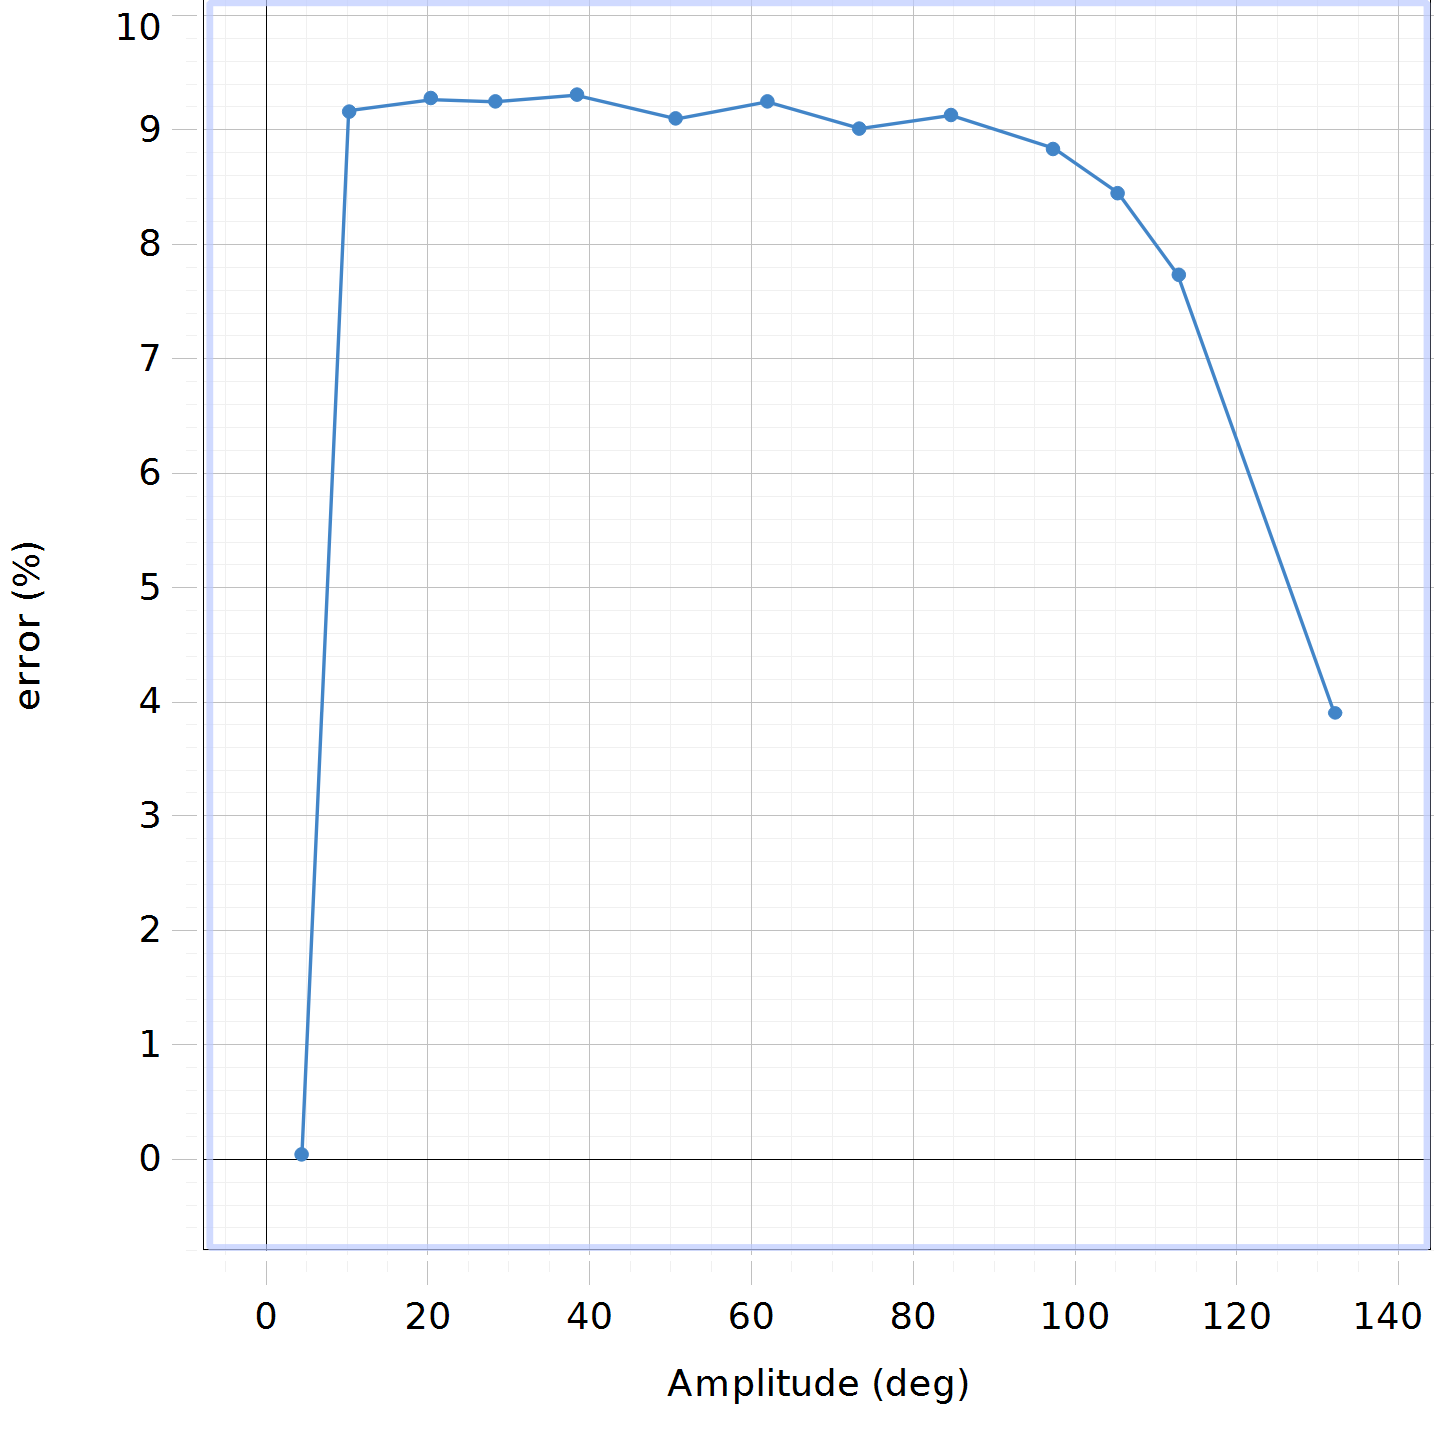
\includegraphics[width=15cm]{figErrorVersusDegree.png}
  \caption{The Error Percentage between Actual and Calculated by Equation \refeq{eq:6} Versus Amplitude Degree}
  \label{figErrorVersusDegree}
\end{figure}
\begin{figure}[H]
  \centering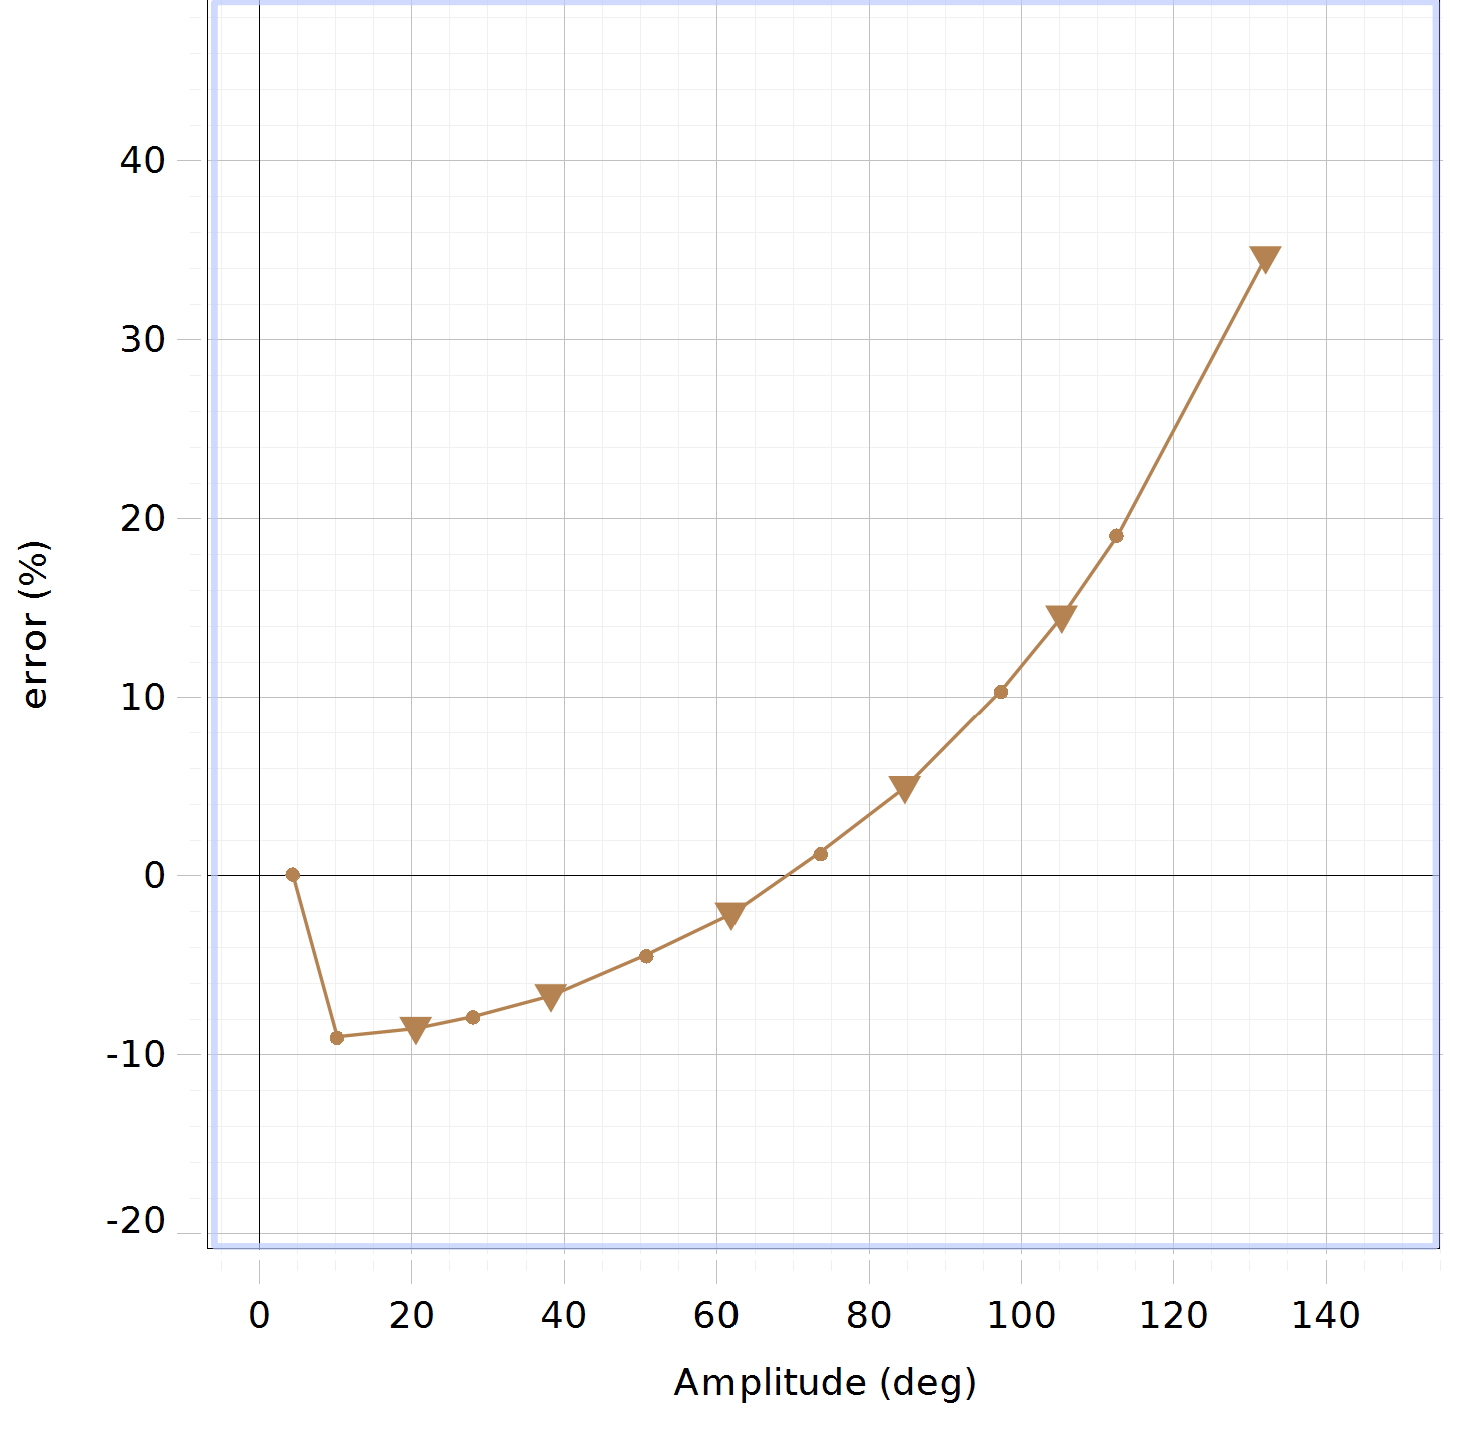
\includegraphics[width=15cm]{figErrorSimp.png}
  \caption{The Error Percentage between Actual and Calculated by Equation \refeq{eq:1} Versus Amplitude Degree}
  \label{figErrorSimp}
\end{figure}
% Tables
\subsection{Raw Data Tables}
\begin{center}
  \begin{tabular}{|c|c|c|c|}
    \hline
    $t_1$(s)        & $t_2$(s)         & Period Zero(s)   & Amplitude(rad)  \\
    \hline
    $4.471\pm0.005$ & $15.432\pm0.005$ & $1.096\pm0.001$ & $0.077\pm0.002$ \\
    \hline
  \end{tabular}
  \captionof{table}{Low Amplitude Period}
  \label{tabLowAmplitude}
\end{center}
\begin{center}
  \begin{tabular}{|c|c|c|c|c|}
    \hline
         & $t_1$(s)         & $t_2$(s)         & Period(s)        & Amplitude(rad)  \\
    \hline
    $1$  & $-1.096\pm0.005$ & $1.096\pm0.005$  & $1.096\pm0.004$ & $0.077\pm0.002$ \\
    \hline
    $2$  & $5.610\pm0.005$  & $7.605\pm0.005$  & $0.998\pm0.004$ & $0.178\pm0.002$ \\
    \hline
    $3$  & $4.035\pm0.005$  & $6.040\pm0.005$  & $1.002\pm0.004$ & $0.358\pm0.002$ \\
    \hline
    $4$  & $3.440\pm0.005$  & $5.460\pm0.005$  & $1.010\pm0.004$ & $0.493\pm0.002$ \\
    \hline
    $5$  & $4.850\pm0.005$  & $6.895\pm0.005$  & $1.022\pm0.004$ & $0.668\pm0.002$ \\
    \hline
    $6$  & $4.660\pm0.005$  & $6.755\pm0.005$  & $1.048\pm0.004$ & $0.886\pm0.002$ \\
    \hline
    $7$  & $5.730\pm0.005$  & $7.875\pm0.005$  & $1.072\pm0.004$ & $1.081\pm0.002$ \\
    \hline
    $8$  & $5.105\pm0.005$  & $7.325\pm0.005$  & $1.110\pm0.004$ & $1.282\pm0.002$ \\
    \hline
    $9$  & $7.960\pm0.005$  & $10.260\pm0.005$ & $1.150\pm0.004$ & $1.478\pm0.002$ \\
    \hline
    $10$ & $7.275\pm0.005$  & $9.695\pm0.005$  & $1.210\pm0.004$ & $1.700\pm0.002$ \\
    \hline
    $11$ & $5.875\pm0.005$  & $8.385\pm0.005$  & $1.255\pm0.004$ & $1.838\pm0.002$ \\
    \hline
    $12$ & $8.565\pm0.005$  & $11.175\pm0.005$ & $1.305\pm0.004$ & $1.967\pm0.002$ \\
    \hline
    $13$ & $6.300\pm0.005$  & $9.250\pm0.005$  & $1.475\pm0.004$ & $2.306\pm0.002$ \\
    \hline
  \end{tabular}
  \captionof{table}{Large Amplitude Period}
  \label{tabLargeAmplitude}
\end{center}

% data and error analysis
\section{Analysis \& Questions:}
\subsection{Error Analysis}
\paragraph{Time}
In all these experiments, we use the embedded clock in PASCO Capstone\texttrademark to measure the time. According to the manual of PASCO Capstone\texttrademark and PASCO 850 Universal Interface, the estimated error of time should be $\pm0.005$s.
\paragraph{Angular Magnitude}
In all these experiments, we use a rotary motion sensor to detect the angular magnitude and angular velocity. According to its official manual, the resolution of this sensor is $0.00157$rad, so we consider its estimated error should be $0.002$rad.\par
Therefore, the columns of estimated data in Table \ref{tabLowAmplitude} and Table \ref{tabLargeAmplitude} have listed raw data with respective estimated error.
\paragraph{Standard Error}
If a function $k$ is determined by $n$ independent random variables, namely $p_1, p_2, ..., p_n$ and $p_i (i=1, 2, ..., n)\sim N(\mu,\sigma^2)$; that is $k=f(p_1, p_2, ..., p_n)$, the standard error for $k$ is given by
\begin{equation}\label{eq:stdErr}
  \delta k=\sqrt{\sum_{i=1}^{n}(\frac{\partial f}{\partial p_i})^2(\delta p_i)^2}
\end{equation}
where $\delta p_i (i=1, 2, ..., n)$ are estimated errors.\par
In Table \ref{tabLowAmplitude}, $t_{\text{period_zero}}=\frac{t_2-t_1}{10}$, by Equation \refeq{eq:stdErr}, we can point out that $\delta t_{\text{period_zero}}=\sqrt{(\frac{1}{10})^2(0.005 \text{s})^2+(\frac{1}{10})^2(0.005\text{s})^2}\approx0.001\text{s}$.\par
In Table \ref{tabLargeAmplitude}, $t_{\text{period}}=\frac{t_2-t_1}{2}$, by Equation \refeq{eq:stdErr}, we can point out that \linebreak $\delta t_{\text{period}}=\sqrt{(\frac{1}{2})^2(0.005\text{s})^2+(\frac{1}{2})^2(0.005\text{s})^2}\approx0.004\text{s}$\par
These calculated estimated standard errors are listed respectively in Table \ref{tabLowAmplitude} and Table \ref{tabLargeAmplitude}.
% TODO
\paragraph{Error from Approximation of Infinite Series}
Let us recall Equation \refeq{eq:5}, which states the relationship between the period and the pendulum amplitude. Approximately, we usually take the first several terms as the result, such as Equation \refeq{eq:6}. Since each term of the infinite series is the product of a square and an even power, our approximation will always smaller than the actual period. If we denote the estimated period time as $T_{\text{est}}$ and the calculated period time from pendulum amplitude as $T_{\text{cal}}$. We can use $\frac{T_{\text{est}}-T_{\text{cal}}}{T_{\text{cal}}}$ to represent the error percentage between theoretical result and actual result under a range of pendulum amplitude, as shown in Figure \ref{figErrorVersusDegree}.

% Data Analysis and Answers
\subsection{Data Analysis \& Questions Answers}
\subsubsection{Qualitative Experiment for Small Angle}

\paragraph{Does the $\theta$ fit a Sine curve as by Equation \refeq{eq:2}?}
We could figure out our answer directly from Figure \ref{figAngleQualitativeSmallAngle}, where RMSE, representing the approximation error, is only $0.00154$. So, the $\theta$ fits the Sine curve as by Equation \refeq{eq:2} perfectly.

\paragraph{Does the \emph{angular velocity} fit a Cosine curve, or a Sine curve as required by Equation \refeq{eq:3}?}
We could figure out our answer directly from Figure \ref{figAngleVelQualitativeSmallAngle}, where RMSE, representing the approximation error, is only $0.00365$. So, the \emph{angular velocity} fits the Sine curve, or the Cosine curve as required in Equation \refeq{eq:3} very well.

\paragraph{Does the \emph{angular acceleration} fit a Sine curve as required by Equation \refeq{eq:4}?}
We could figure out our answer directly from Figure \ref{figAngleAccelQualitativeSmallAngle}, where RMSE representing the approximation error, is $0.0145$. So, the \emph{angular acceleration} fits the Sine curve as required in Equation \refeq{eq:4} quite well.

\paragraph{What does the minus sign in Equation \refeq{eq:4} do?}
In fact, it is the gravity acting as resistance when the rod is raising up. By Newton's Second Law of Motion $F=ma$, considering the positive direction of \emph{linear velocity}, gravity is at obtuse angle with it. So the gravity is acting as resistance and should put a minus sign on $F$ to represent the opposite direction. This leads to $a$ acting as minus \emph{linear acceleration}. As \emph{linear} ones are corresponding to \emph{angular} ones, so there is a minus sign in Equation \refeq{eq:4}.

\paragraph{Are the periods of the three curves the same?} Yes, they are. Theoretically, from Equation \refeq{eq:2}, Equation \refeq{eq:3} and Equation \refeq{eq:4}, we can point out that the periods are all determined by $\omega$ and exactly same. From the perspective of experiment, we could compare Figure \ref{figAngleQualitativeSmallAngle}, Figure \ref{figAngleVelQualitativeSmallAngle} and Figure \ref{figAngleAccelQualitativeSmallAngle}. We could state that for their respective approximate Sine curves, $\omega$ is at the same value. So, the period determined by $\omega$ is the same.

\subsubsection{Qualitative Experiment for Large Angle}

\paragraph{Do the \emph{angular velocity} and \emph{angular acceleration} data fit a Sine curve as required by Equation \refeq{eq:3} \& \refeq{eq:4} from Theory?}
No. Compare Equation \refeq{eq:1} and Equation \refeq{eq:5}, we will find out the former one is the approximation of the latter one under circumstance of small pendulum amplitude. Equation \refeq{eq:2}, \refeq{eq:3} and \refeq{eq:4} is the corollary from Equation \refeq{eq:1}. Therefore, they do not meet with the circumstance of large pendulum amplitude.

\paragraph{Why do the places where the speed is zero correspond to turning points where the displacement is maximum?}
When the displacement is maximum, the mass is at its highest place, where its speed is changing from towards up to towards down, that is, the speed of raising part is descending until it reaches its highest position and begin to fall. Mathematically, speed is the derivative of displacement over time, when Sine curve comes to its maximum or minimum, its derivative, the Cosine curve should be zero.

\paragraph{Why do places where the speed is maximum correspond to places where both the displacement and acceleration are zero?}
When the speed is maximum, the mass should be its lowest place, where it is falling to increase the speed and it is going to raise to decrease the speed, that is, the gravitational potential is fully transferred into kinetic energy. So, the displacement is zero. When the displacement is zero, the gravity is perpendicular to the \emph{linear velocity}. Therefore, the gravity offers no acceleration on \emph{linear velocity}'s direction. Then, the \emph{angular acceleration} should be zero.

\paragraph{We observe double peaks with a valley in between in the acceleration curve. What does this correspond to in the velocity curve? }
When the gravity is perpendicular to the rod, the gravity is parallel to the \emph{linear speed} and gives the largest \emph{linear acceleration}, leading to the largest \emph{angular acceleration}. However, under the circumstance of large amplitude pendulum, the rod may raise over $90^\circ$. Then, the gravity will perpendicular first and then cross as a acute angle, making the \emph{sub-Force} acting on the direction of the \emph{linear speed} descend. Therefore, the \emph{linear acceleration} descend and so the \emph{angular acceleration}.

\subsubsection{Quantitative Experiment}

\paragraph{Why is the expansion in Equation \refeq{eq:5} including only first two terms enough to match the data well for angles which are less than \boldmath{45}$^\circ$ (about \boldmath{0.8}rad)?}
We can use $\frac{T_{\text{est}}-T_{\text{cal}}}{T_{\text{cal}}}$ to represent the error percentage between theoretical result and actual result. While the second term contributes $\frac{(\frac{1}{2})^2\sin^2(\frac{45^\circ}{2})}{1+(\frac{1}{2})^2\sin^2(\frac{45^\circ}{2})}\times100\%\approx4\%$, the third term contributes only $\frac{(\frac{3\times1}{2^2\times2\times1})^2\sin^4(\frac{45^\circ}{2})}{1+(\frac{1}{2})^2\sin^2(\frac{45^\circ}{2})+(\frac{3\times1}{2^2\times2\times1})^2\sin^4(\frac{45^\circ}{2})}\times100\%\approx0.302\%$. We can consider that the error cause from third term and so on are less crucial than the estimated error caused by equipment.

\paragraph{Why does the approximation begin to fail for angles above \boldmath{90}$^\circ$ (about \boldmath{1.57}rad) even when we include first five terms in the approximation?}
Similarly to the last question, consider the contribution of error diminution of the sixth term. It contributes \linebreak $\frac{(\frac{63}{256})^2\sin^{10}(\frac{90\circ}{2})}{1+(\frac{1}{2})^2\sin^2({\frac{90\circ}{2}})+({\frac{3}{8}})^2\sin^4({\frac{90\circ}{2}})+({\frac{15}{48}})^2\sin^6({\frac{90\circ}{2}})+({\frac{105}{384}})^2\sin^8({\frac{90\circ}{2}})+(\frac{63}{256})^2\sin^{10}(\frac{90\circ}{2})}\times100\%>1\%$. It exceeds our expected error $1\%$.

\paragraph{How many terms would be required for the approximation to give a good value for the case where the amplitude equals $3.0$ rad?}
Since we do not collect the actually experimental data for $3.0$rad, we use the difference of consecutive two terms to represent its accuracy. Using a \hyperref[Python]{Python program} to calculate, then we find with the consecutive two terms different in $0.00001$ we need at least 152 terms.

\paragraph{Assume the \emph{Simple Harmonic Oscillation} period given by Equation \refeq{eq:1} was applied to all amplitudes. How large is the error at an amplitude of \boldmath{20}$^\circ$ and \boldmath{40}$^\circ$?}
We can take a careful observation on Figure \ref{figErrorSimp}. With amplitude$=20^\circ$, the error is about $8.6\%$, while it is about $6.5\%$ when the amplitude goes $40^\circ$.

\section{Conclusion}
By conducting the experiments, we finally find out the the function curve of displacement, angular velocity and angular acceleration under small amplitude pendulum. Then, we also point out that these curves do not meet with the fact when it is under the circumstance of large amplitude pendulum. Therefore, we introduce the \hyperref[eq:5]{infinite series} to manage to describe the fact more precisely. To examine its effect, we compare the actual data with these two kinds of theoretical data. The result is satisfied. While the calculated from Equation \refeq{eq:1} lead to a big error, the new method, the \hyperref[eq:5]{infinite series} matches the experimental data with small error only with first several terms. Therefore, we are now clear the mathematical model of both small and large amplitude pendulum.
\pagebreak

\section*{Appendix}
\lstinputlisting[
    style       =   Python,
    caption     =   {\bf calculate.py},
    label       =   {Python}
]{calculate.py}


\end{document}
